%%% intro on CERN and LHC 
%%% goals of particle physics research at CERN

\chapter{The LHC and the ATLAS experiment}%\label{chap:LHC_ATLAS}

The theory that currently best describes the fundamental particles and their interactions is known as the Standard Model \cite{Herrero1999}. It was developed during the 20th century and finalized in the mid-1970s, after experimenal confirmations of quarks. The Standard Model has since predicted and explained a wide range of phenomena with great accuracy, important examples are the W and Z bosons and the Higgs boson. However, some questions still remain unanswered.


\section{The Large Hadron Collider}
\begin{figure}[!ht]
    \centering
    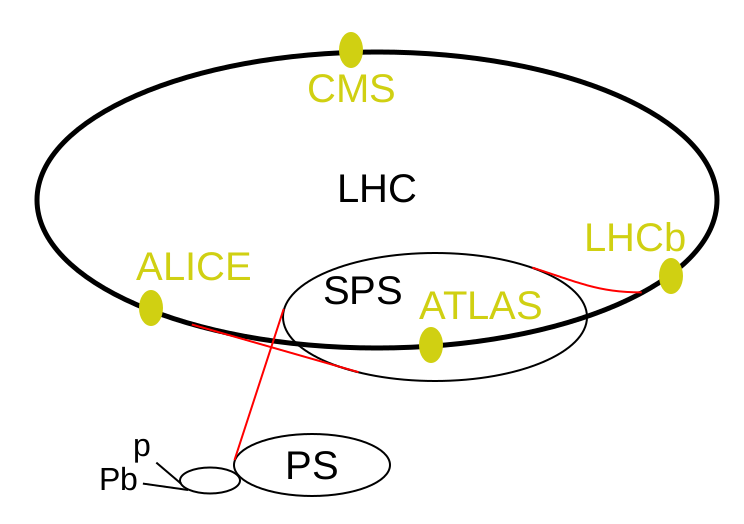
\includegraphics[width=.7\linewidth]{Images/intro/LHC.png}
    \captionsetup{width=.7\linewidth}
    \caption{Simplified scheme of the CERN accelerator complex. Each proton or lead ion starts from a linear accelerator (LINAC 4 and LINAC 3, respectively, not in the picture), it is then transferred to the Proton Synchrotron (SP), into the Super Proton Synchrotron (SPS) and finally into the Large Hadron Collider (LHC). During each phase of acceleration the particles reach higher momentum before being transferred to the next stage.}
    \label{fig:LHC}
\end{figure}

\marginpar{\flushleft I could add some details of the process of acceleration, from H atoms to proton beam into the LHC}

The Large Hadron Collider (LHC) is the largest particle accelerator in the world. It was built between 1998 and 2008 by the European Organization for Nuclear Research (CERN, \textit{Conseil européen pour la Recherche nucléaire}) in collaboration with more than 100 countries with the purpose of colliding hadrons\footnote{\label{footnote:hadrons}Hadrons are particles that are made up of two or more quarks, e.g. protons and neutrons} at high energies and study the products of these collisions. It consists of a \qty{27}{\kilo\meter} ring at roughly \qty{100}{\meter} of depth situated at the Franco-Swiss border, near Genève. Two beams of particles travel at near light speed in opposite directions inside two pipes surrounded by superconducting magnets. At specific locations the beams converge and collisions take place, these events can then be observed with specialized detectors built along the tracks.


\subsection{The research goals}%\label{sec:CERN_research_goals}

The construction of the LHC was motivated by the need for experimental data to study the laws of our universe. In particular, its main research goals were \cite{homeFactsFigures}:
\begin{itemize}
    \item The search for the Higgs boson, the particle (whose mass could not be predicted) responsible for the origin of mass, culminated in the discovery of the Higgs boson in 2012 \cite{20121}. 
    \item Supersymmetry, a theory that hypothesizes the existence of massive partners of the particles in the current Standard Model.
    \item Dark matter and dark energy, the matter that we know only makes up a small fraction, \~4\%, of the content of the universe, and the particles or phenomena responsible for the remaining 23\% (dark matter) and 73\% (dark energy) are still unknown.
    \item Matter-antimatter asymmetry, matter and antimatter should have been produced in identical amounts during the Big Bang, but so far we have observed almost exclusively normal matter.
    \item Quark-gluon plasma, the state of matter before ordinary matter could emerge in the early stages of the Universe.
\end{itemize}

The LHC is part of the CERN accelerator complex, a chain of machines in which each link accelerates a beam of particles (protons or heavy ions) to higher energies and feeds it to the next one. A simplified version of the complex is shown in Figure \ref{fig:LHC}. The LHC began operations in 2010 with energies of \qty{3.5}{\tera\electronvolt}, increased up to \qty{4}{\tera\electronvolt} in 2012. After two years of Long Shutdown for upgrades and maintenance, activities resumed in 2015 with Run 2, when beam energies of \qty{6.5}{\tera\electronvolt} ($\sqrt{s}=\qty{13}{\tera\electronvolt}$, center of mass energy) were achieved.


\subsection{The main experiments}\label{subsec:LHC_main_experiments}

Along the accelerator tracks there are four main experiments (Figure \ref{fig:LHC}):
\begin{itemize}
    \item ALICE (A Large Ion Collider Experiment), dedicated to heavy-ion physics\cite{homeALICE}.
    \item ATLAS (A Toroidal LHC Apparatus), one of the two general-purpose detectors, able to investigate a wide range of physics.
    \item CMS (Compact Muon Solenoid), the second general purpose detector of LHC.
    \item LHCb (Large Hadron Collider beauty), an asymmetric detector that observes mainly forward particles to study the "b quark".
\end{itemize}

Additionally, there are several other experiments part of the CERN complex, including test beam facilities in the North Area which use a particle beam from SPS to perform a variety of tests.

\begin{figure}[!ht]
    \centering
    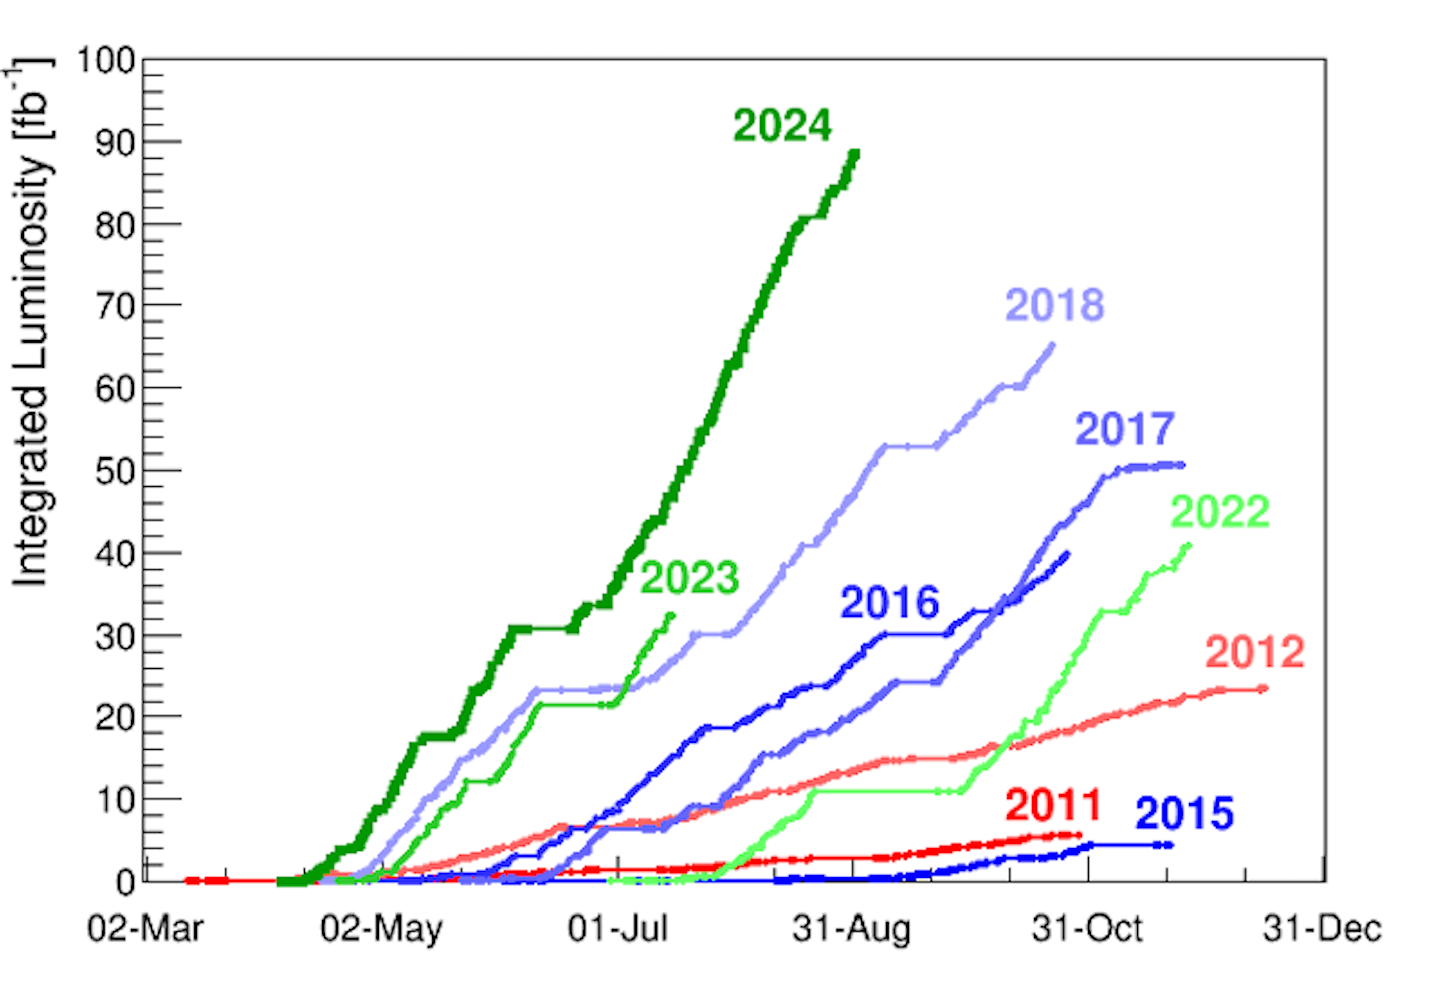
\includegraphics[width=.6\linewidth]{Images/intro/integrated_luminosity.png}
    \captionsetup{width=.8\linewidth}
    \caption{Overview of the integrated luminosity as a function of the date for each year of LHC running, with 2024 greatly exceeding all other years. From \cite{homeAcceleratorReport}.}
    \label{fig:integrated_luminosity}
\end{figure}

One of the most important parameters of a collider, along with the beam energy, is the luminosity. It is used to quantify the amount of interactions that will occur and, therefore, the expected rate of events produced by the collisions. For two bunches\footnote{\label{footnote:particle_beam_bunches} The particles in the LHC beam do not travel uniformly distributed, rather they are grouped in many \textit{bunches}, synchronized to intersect at the center of each main detector (Section \nameref{subsec:LHC_main_experiments}).} colliding head-on with frequency $f_{coll}$, the luminosity can be calculated by:

\begin{equation}
    \mathcal{L} = f_{coll}\frac{N_1 N_2}{4\pi \sigma_x \sigma_y} \mathcal{F} \, \left[\unit{cm^{-2}.s^{-1}}\right] \, .
\end{equation}

Where $N_1$ and $N_2$ are the number of particles in each bunch, $\sigma_x$ and $\sigma_y$ define the transverse spread of the bunches (approximately Gaussian distributions) at the interaction point, and $\mathcal{F}$ is factor of order $1$ to account for inefficient geometric overlapping and other effects.

A related quantity is the integrated luminosity, which is the integral over time which quantifies that amount of data that is available to be studied, typically measured in inverse femtobarns \unit{\femto\barn^{-1}}=\qty{e-28}{\meter^{-2}}.

After the second Long Shutdown that took place between 2018 and 2022 LHC has been operating (Run 3), and delivering already record breaking integrated luminosity (Figure \ref{fig:integrated_luminosity}).

%%% plans for the next years
\subsection{High-Luminosity upgrade}\label{subsec:high_luminosity_upgrade}
In the upcoming years there will be a third Long Shutdown (from around 2026,until early 2029) to prepare for the next phase: the High-Luminosity LHC Project (HL-LHC) \cite{cernHLLHCProject}. The plan aims to increase the instanteous luminosity up to \qty{1.5e34}{\centi\meter^{-2}\second^{-1}} (compared to \qty{2.1e34}{\centi\meter^{-2}\second^{-1} of Run 2} \cite{CERN-LHCC-2020-007}) and to bring the integrated luminosity up to \qty{3000}{\femto\barn^{-1}} in the following 10-12 years. This will enable more accurate measurements of new particles and the possibility to observe rare processes below the current sensitivity level. On the other hand, this upgrade will introduce a wide range of new challenges for all the systems within CERN's accelerator complex. For instance, the detectors will be exposed to higher radiation doses, which may impact performance, and the increased number of collisions will lead to more pronounced pile-up effects complicating track reconstruction.

% this is already kinda talking about HGTD, maybe it's a good bridge to the next section: HGTD
\begin{figure}[!ht]
    \centering
    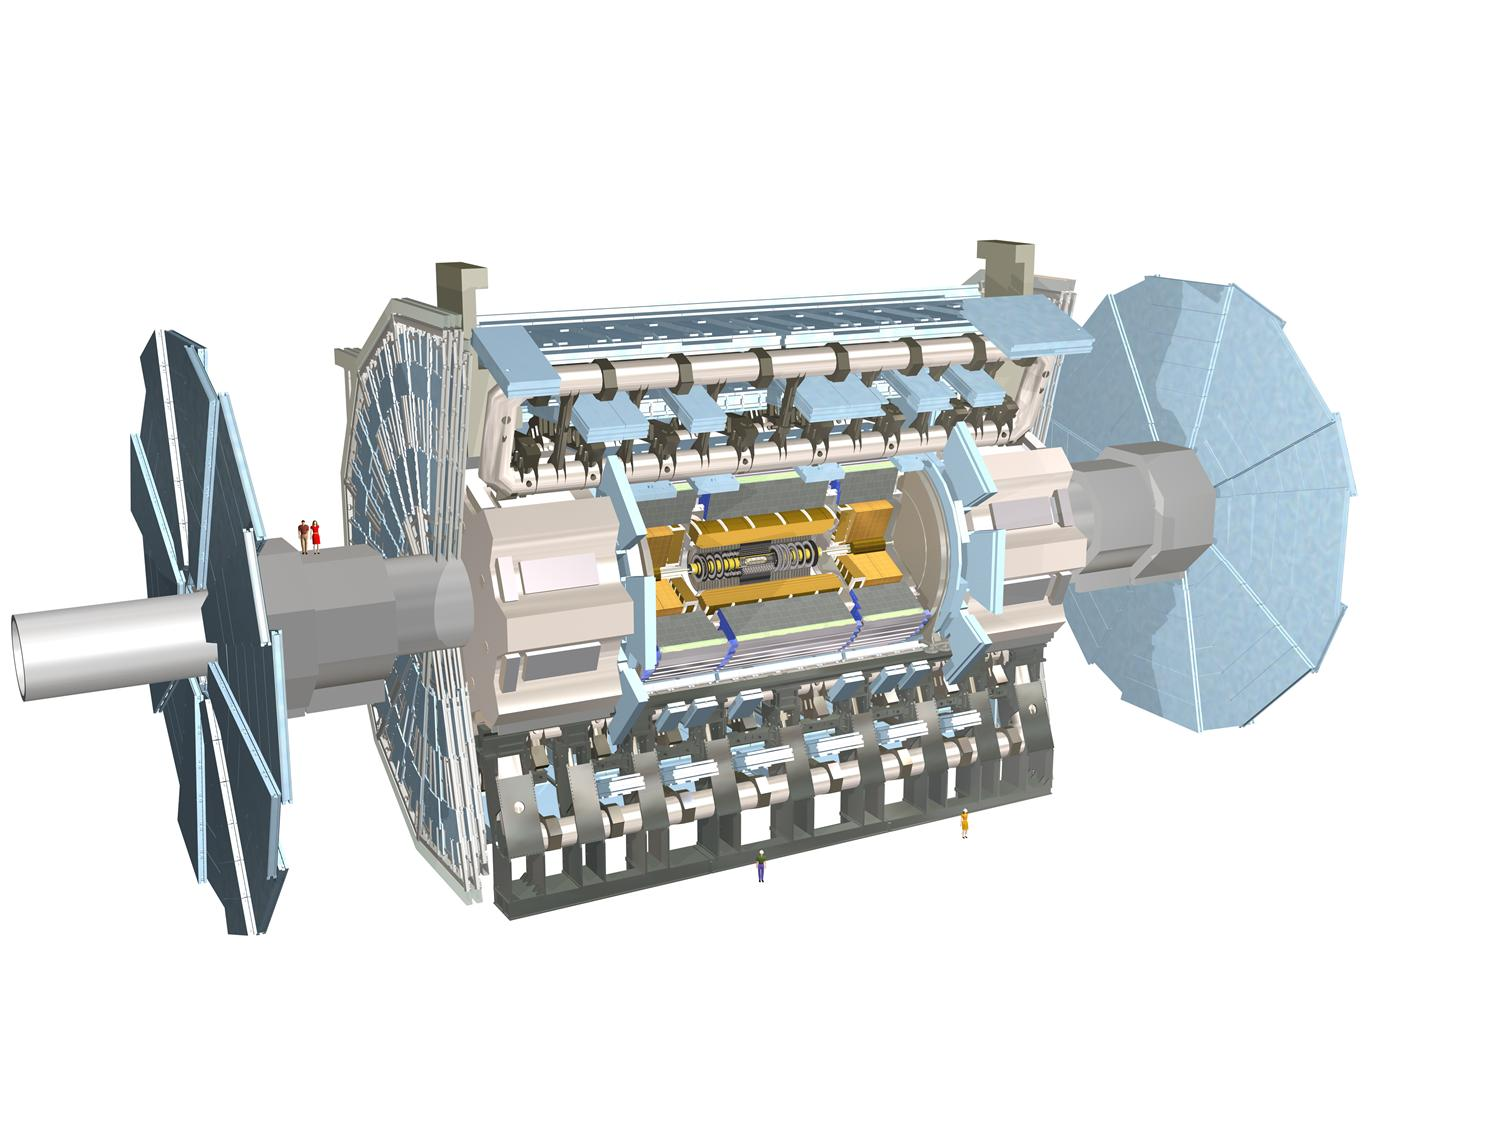
\includegraphics[width=.7\textwidth]{Images/intro/ATLAS_detector.jpg}
    \captionsetup{width=.8\linewidth}
    \caption{Overview of the ATLAS detector. From \cite{atlasDetectorTechnology}}
    \label{fig:ATLAS}
\end{figure}


\section{The ATLAS experiment}%\label{chap:ATLAS}

ATLAS (\textbf{A} \textbf{T}oroidal \textbf{L}HC \textbf{A}pparatu\textbf{S}) is a general purpose detector built for probing \textit{p-p} and \textit{A-A} collisions (\textit{proton-proton} and \textit{heavy ion-heavy ion}, respectively). Currently, the experiment's main detector systems are: the Inner Detector, the Calorimeters, the Muon Spectrometer and the Magnet System \cite{Collaboration_The_ATLAS2008}. 

\begin{figure}[hb]
    % \centering
    % \subfloat[Radial view of the ATLAS Inner Detector. From \cite{atlasInnerDetector}]{
    %     \includegraphics[width=.48\linewidth]{Images/intro/ATLAS_inner_detector_radial_description.jpg}
    %     \label{fig:ATLAS_inner_detector_radial}}
    % \hfill
    \centering
    \subfloat[The Inner Detector and its three components: the Pixel Detector, the Semiconducor Tracker and the Transition Radiation Tracker. From \cite{atlasInnerDetector}]{
        \includegraphics[width=.45\linewidth]{Images/intro/ATLAS_inner_detector.jpg}
        \label{fig:ATLAS_inner_detector}}
    \hfill
    \centering
    \subfloat[The Calorimeters: the Liquid Argon Calorimeter (LAr) and Tile Hadronic Calorimeter]{
        \includegraphics[width=.45\linewidth]{Images/intro/ATLAS_calorimeter_description.jpg}
        \label{fig:ATLAS_calorimeter}}
\end{figure}


\subsection{Inner Detector}\label{sec:ATLAS_inner_detector}
\marginpar{\flushleft }
The main purpose of the Inner Detector is to reconstruct the verteces of the collisions, it comprises three sub-detectors (Figure \ref{fig:ATLAS_inner_detector}).

The Pixel Detector is the first point of detection, only \qty{3}{\centi\meter} away from the LHC beam line and it is made of four layers of silicon pixels, more than 92 million in total. Charged particles originated from the collision points leave a small amount of energy that can be measured by the pixels with a precision of almost \qty{10}{\micro\meter}. These signals are then used to reconstruct the origin and the momentum of the particle.

The Semiconducor Tracker sorrounds the Pixel Detector and complements it detecting and reconstructing the tracks of charged particles. It consists of over 6 million "micro-strips" silicon detectors with a precision of up to \qty{25}{\micro\meter}.

The final layer of the Inner Detector is the Transition Radiation Tracker (TRT). Unlike its neighbouring silicon sub-detectors, TRT is composed of \num{300000} of \qty{4}{\milli\meter} diameter tubes with a \qty{30}{\micro\meter} gold-plated tungsten wire in the centre and filled with a mixture of gas. As charged particles pass through the volume they ionize the gas, which creates detectable electric signals. The location can then be determined, helping with the tracks reconstruction and the momentum measurement. Additionally, the moving particles emit transition radiation\footnote{Transition Radiation occurs when a charged particle traverses materials with different refraction index, such as the boundary between two different media \cite{wikipediaTransitionRadiation}.}, and the intensity of this radiaiton depends on the $\gamma$ Lorentz factor, thus allowing to distinguish between heavier and lighter particles.


\subsection{Calorimeter}\label{sec:ATLAS_calorimeter}

% \begin{figure}[!ht]
%     \centering
%     \includegraphics[width=.8\textwidth]{Images/intro/ATLAS_calorimeter_description.jpg}
%     \captionsetup{width=.8\linewidth}
%     \caption{Layout of the components inside the Calorimeter. From \cite{atlasCalorimeter}}
%     \label{fig:ATLAS_calorimeter}
% \end{figure}

Calorimeters are designed to absorb most of the incoming particles, forcing them to deposit all of their energy and stop within the detector. Electromagnetic calorimeters (ECAL) measure the energy of electrons and photons while they interact with matter via electromagnetic force. Hadronic calorimeters on the other hand measure the energy of hadrons (footnote\footref{footnote:hadrons}) as they interact with atomic nuclei via strong force. Calorimeters can stop most known particle, with the exception of muons (see Section \ref{sec:muon_spectrometer}) and neutrinos.

The ATLAS calorimetry system has two components: the Liquid Argon Calorimeter (LAr) and the Tile Hadronic Calorimeter

The Liquid Argon Calorimeter (LAr) features layers of metal (either tungsten, copper or lead), with liquid argon in-between, kept a temperature of \qty{-184}{\degreeCelsius}. Several modules are placed cylindrically around the beam (the barrel) and at the extremities (endcaps).

The Tile Hadronic Calorimeter surrounds the LAr calorimeter, it has the goal of measuring hadronic particles that did not deposit all of their energy in the LAr. It consists of alternating layers of steel and plastic scintillating tiles. Particles hitting the steel layer create a shower of other particles, the plastic scintillators in turn produce photons, which are then converted into an electric current to determine the original particle's energy.


\subsection{Muon Spectrometer}\label{sec:muon_spectrometer}

The outer layer of the ATLAS experiment is composed of muon\footnote{Muons are particles similar to electrons but \~200 times heavier. This allows them to penetrate much deeper into matter, due to less emitted radiation as they decelerate.} detectors, which identify and measure the momenta of muons. Five different detector technologies employed separated into two categories: Fast-Response Detectors, to quickly select collisions potentially interesting for physics, and Precision Detectors, to provide very precise positions of muons.

In the first group there are: 
\begin{itemize}
    \item Resistive Plate Chambers (RPCs), surrouding the central region of ATLAS. They are pairs of parallel plates at an electric potential difference, separated by gas.
    \item Thin Gap Chambers (TGCs), found at the ends of ATLAS. They consist of \qty{30}{\micro\meter} parallel wires in a gas mixture.
\end{itemize}
Both of these detectors measure the electric signals of particles as they ionize the gas. Additionally, there two dectors\cite{KOULOURIS2020162757} specially designed for the High Luminosity upgrade, to be placed on either side of the detector, very close to the beam pipe:
\begin{itemize}
    \item Micromegas (MicroMEsh GAseous Structure), which will serve as primary tracking detector.
    \item Small-Strip Thin-Gap Chambers (sTGCs), which will function as primary trigger detector.
\end{itemize}

Finally, for the role of Precision Detectors, Monitored Drift Tube (MDTs) are able to determine the position of a muon to an accuracy of \qty{100}{\micro\meter}. They are consituted by more than \num{380000} aluminium tubes with a wire at the tube's center and filled with a gas mixture. They are stacked up over several layers, to precisely trace the path of each muon.


\subsection{Magnet System}\label{sec:magnet_system}

\begin{figure}[!ht]
    \centering
    \subfloat[The Central Solenoid Magnet at its installation, 2004. From \cite{atlasMagnetSystem}]{
        \includegraphics[width=.45\linewidth]{Images/intro/ATLAS_central_solenoid_magnet.JPG}
        \label{fig:ATLAS_central_solenoid}}
    \hfill
    \centering
    \subfloat[The installation of the eighth and final coild of the Barrel Toroid Magnet, 2005. From \cite{atlasMagnetSystem}]{
        \includegraphics[width=.45\linewidth]{Images/intro/ATLAS_barrel_toroid_magnet.JPG}
        \label{fig:ATLAS_barrel_toroid}}
\end{figure}

Using magnets, the trajectories of charged particles can be bent, allowing the calculation of their momentum and charge. In ATLAS this is done two different types of superconducting magnet systems: toroidal and solenoidal, utilized in the three main sections: Central Solenoid Magnet, Barrel Toroid and End-cap Toroids.
\begin{itemize}
    \item Central Solenoid Magnet, it surrounds the inner detector at the core of ATLAS. It provides a \qty{2}{\tesla} magnetic field in just \qty{4.5}{\centi\meter} thickness (Figure \ref{fig:ATLAS_central_solenoid}).
    \item Barrel Toroid, the largest toroidal magnet ever constructed, providing a magnetic field of up to \qty{3.5}{\tesla}. It is used to measure the momentum of muons.
    \item Two End-cap Toroids, placed at each end of the experiment. They extend the magnetic field to particles escaping the detector close to the beam pipe.
\end{itemize}

\subsection{The upgrades}\label{subsec:ATLAS_upgrades}

Short overview of the changes that ATLAS will undergo, most importantly:

- ITk replacing the Inner Detector
- new HGTD installed

